%!TEX root = ../dissertation.tex

\chapter{The Algorithm} \label{cha:algorithm}

%%The purpose of this project is to show how a proto-AGI system such as OpenCog can be used 
Having defined the OpenCog system and part of the implementation of the problem in the previous chapters, it is now possible to combine all the various modules and explain the functioning of the internal design and the main algorithm. \\

It is possible to divide the entire project into 6 phases: initial, perception, learning, request, search and results execution.  

\section{Initial Phase}\label{sec:init}

The initial phase concerns the initialization of the simulated environment. The framework used for the development and programming of the robot is the well-known ROS, Melodic version, and the Gazebo 9 system handles the simulation. \\
Therefore, the world as in Figure \ref{fig:env_2_named} is loaded into Gazebo. 
It consists of a robot manipulator with an attached camera, some fixed objects (such as tables, shelves, etc.) and cubes, both with their AprilTags used for detection and semantic assignment. \\
Then, a server in C++ code is activated and the nodes of the ROS system for robot control and object perception become available for listening. \\
Finally, the main AtomSpace is created and the actions rules are loaded into it. 

\begin{figure} [h]
\centering
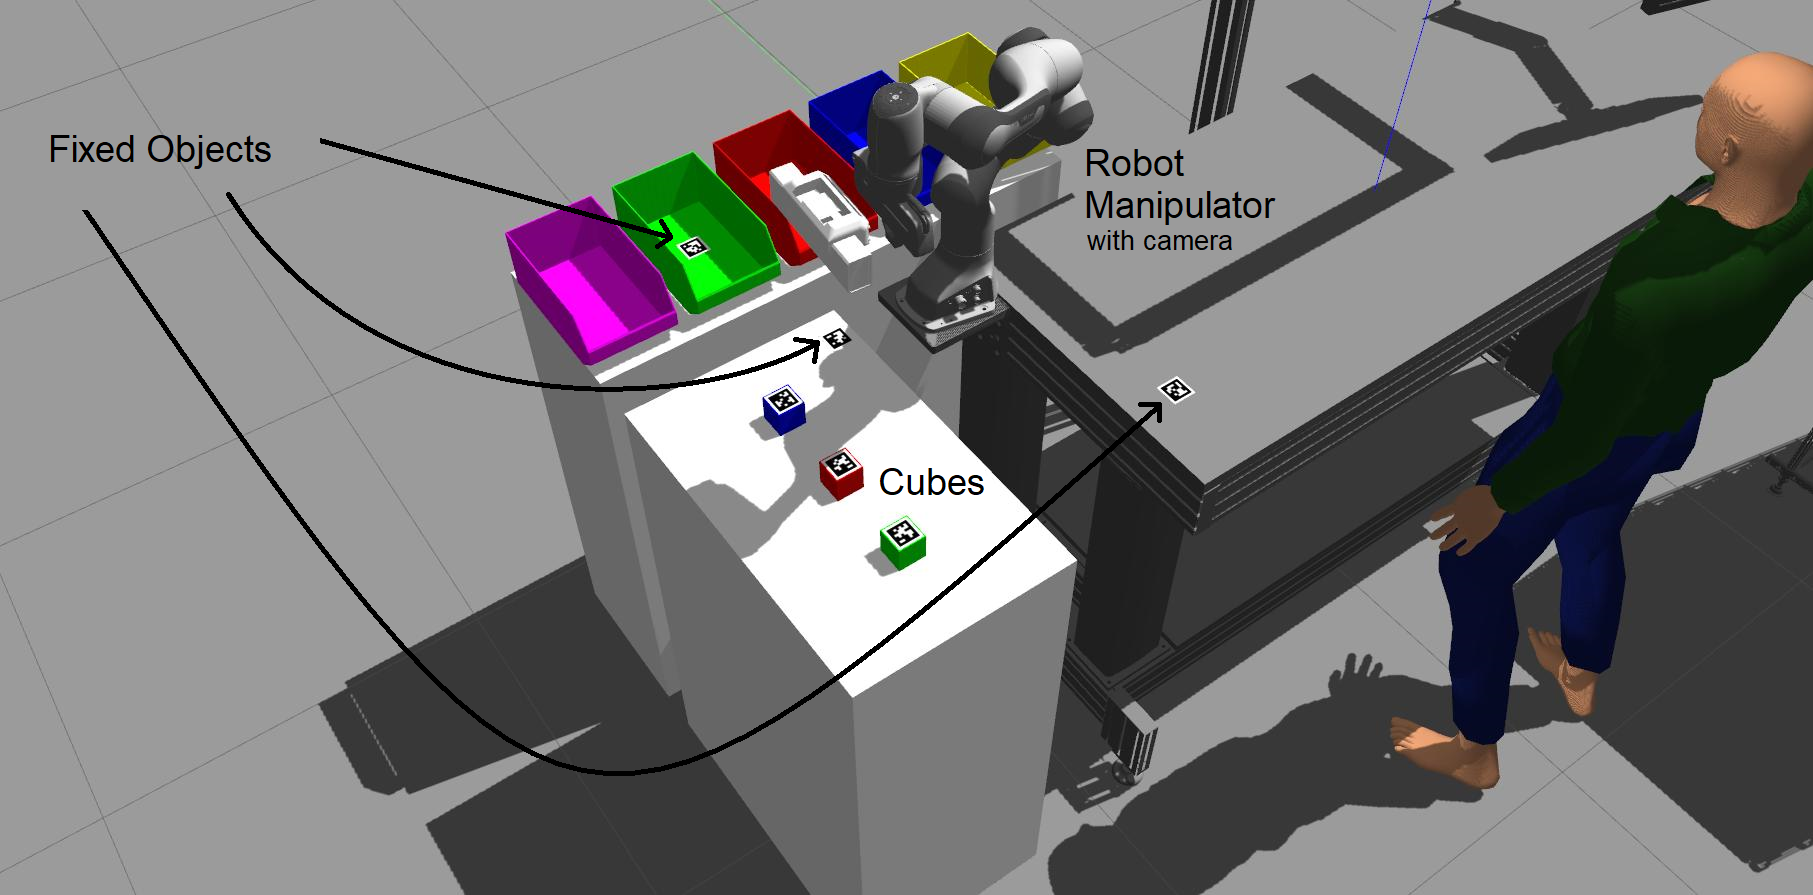
\includegraphics[width=0.9
\textwidth]{figures/Magistrale/env_2_named}
\caption[Environment Components]{ TODO: descrizione
\label{fig:env_2_named}}
\end{figure} 

\section{Perception Phase}\label{sec:perception}

The perception phase, like the remaining phases, is written in Python code and sends commands via a Python client to the C++ server mentioned above. These commands move the robot and allow it to scan its surroundings area for possible objects (related AprilTags are recognised), thanks to the camera attached to the top of it. \\
Of each AprilTag found, its associated semantic representation (i.e. English word describing the object, as well as the name of its relative ConceptNode) is returned by the server to the client, which in turn returns it to the main Python code that begins the initialization of the objects list present in the environment.

\section{Learning Phase}\label{sec:learning}

The learning phase is used to provide additional information. \\
The perception algorithm is extremely simple and does not deal with information processing. Consequently, it is not able to distinguish an object from a fixed object or to infer that an object is placed on top of another. Surely, with a perception processing module all of this, and much more, could be managed. \\
However, this project shows the simplicity of integration and the potential of the learning with the OpenCog system. \\

This phase was created to tell the robot which objects are fixed and which objects are on top of others (fixed objects excluded) or which object is in the robot's hand. That is, to provide the necessary additional information, which the simple perception phase does not perceive, to describe the initial situation of the environment.
This is done by a module using NLP, consisting of the Relex2Logic OpenCog module and a post-processing phase. \\

Additional information is provided to the system via English sentences. \\
This module applies Relex2Logic to these sentences, creating the hypergraph describing them within a new empty AtomSpace (as explained in Section \ref{sec:r2l}).  \\
Next, the post-processing phase loads the rules set out in Section \ref{sec:NLP} and executes them within that AtomSpace. Those rules look for patterns corresponding to the possible information that the system might need and create summary atoms that can be easily used by the algorithm. Thus, from the results obtained by Relex2Logic, they infer atoms such as the ones shown in Section \ref{sec:env_atomese}, which are then added to the main AtomSpace. \\

Moreover, from the information learned in this phase, the \textit{clear} state atoms of the effectively free objects and the \textit{object} inheritance atoms of the non-fixed objects are created.  \\
Finally, the last atoms of the initial KB are added to the main AtomSpace. They are all possible simple combinations (without repetition) from the objects list taken two at a time (explained in Section \ref{sec:r2l}, too). \\
The main AtomSpace is now complete and fully describes the initial situation. 

\section{Request Phase}\label{sec:request}

The request phase behaves like the previous one, except for the aim. Whereas before, English sentences are used to give additional information, now new English sentences are requested to define the goal to be achieved. \\
In order to define the goal it is not necessary to describe the final complete arrangement of objects in the environment, but simply the states of the objects one wants to achieve. \\
Thus, the same steps used in the learning phase are performed here. That is, the English sentences are processed to obtain the corresponding set of atoms that describes them. Then, these atoms are added to a goal list used by the algorithm to find a solution.

\section{Search Phase}\label{sec:search}

The search phase is the core of the algorithm and tries to achieve an arrangement of objects in which all atoms in the goal list are satisfied.
To find a solution, the AtomSpace of the final arrangement must contain every atom within the goal list. \\

Since each atom is unique in the AtomSpace, two AtomSpaces describing the same arrangement and state of objects have the same atoms, thus they are identical. 
Consequently, each possible arrangement of objects in the environment can be associated with one and only one AtomSpace, making it a de facto state of a Finite State Machine (FSM).
Moreover, each of the four actions available to the robot can be seen as a step of this FSM. 
Starting from a certain state, performing an action leads that state (i.e. that AtomSpace) into a new one. However from each state, one or more actions can be performed and thus, one or more states can be reached. \\

One of the best ways to handle this structure is through a tree that has AtomSpaces as tree-nodes (to distinguish them from Nodes in Atomese) and available actions as tree-edges. 
After the request phase, the root of the tree, containing the main AtomSpace, is created. \\
Next, a search algorithm, based on the well-known Breadth-First Search (BFS) (more details in \cite{BFS-wiki, BFS}), expands the tree in search of a solution.

\subsection{BFS-Based Algorithm}\label{sec:bfs_search}

The BFS-based algorithm is recursive and accepts as arguments a tree-node and a variable, which limits the actions to be performed. \\
Following the rules of the problem (Secion \ref{cha:problem_description}), it is trivial to deduce that the actions alternate for each step of the algorithm.
That is, starting from the root:

\begin{enumerate} 
	\item If there exists an atom, within the AtomSpace contained in the root, that describes the \textit{in-hand} state of an object, then only \textit{Stack} and \textit{Putdown} actions can create childs. Conversely, if there are no objects in hand, only the actions of \textit{Pickup} and \textit{Unstack} can. This is because the current state of the robot's hand limits the action used to go to the next state. If the hand is free, it can only grab an object, while if it is busy, it can only place the object down.

	\item From this first intuition, follows the one applicable to each step: given a certain tree-node, if the action that created it is \textit{Stack} or \textit{Putdown}, then the childs of that node can only be created by \textit{Pickup} or \textit{Unstack} actions, and vice versa.
\end{enumerate}

This is why the BFS-algorithm has a variable as the second argument, it holds the action used to create the node in the first argument. \\
Trying all actions at each step would also achieve the same result, as unavailable actions would still give a null result, but this way speeds up the algorithm and avoids unnecessary code execution.


\subsubsection{Termination Criteria of the BFS-Based Algorithm}\label{sec:term_criteria}

Some additional parameters are defined to limit and improve the search. As a result, it is possible to use 4 different searches:

\begin{enumerate}
	\item Search until a first solution is found
	\item Search restricted to a maximum number of iterations 
	\item Explore the whole tree
	\item Quick search
\end{enumerate}

The quick search finds a solution, decreasing the number of iterations in most situations.
As this type of problems suffers from combinatorial explosion\footnotemark{}, the number of tree-nodes grows exponentially as the tree expands.
\footnotetext{\url{https://en.wikipedia.org/wiki/Combinatorial_explosion}} \\
One way to reduce this expansion is to limit the available actions to only those that interact with one or more objects appearing in the goal list.
Many unnecessary actions are avoided, however this makes the algorithm incorrect, since the certainty of finding a solution is lost.
It still works well for most initial arrangements and goal lists and if it fails, the search in step 1 (which is correct, like search 2 and 3, if a solution exists) can be used. \\

Finally, a solution is found when all the atoms composing the goal list are within the AtomSpace of a node. \\
Furthermore, the first solution found will certainly be the optimal solution, i.e. the solution that uses the minimum number of actions to go from the initial arrangement of objects to the goal one.
This is because for each tree-node, before being expanded, its AtomSpace is compared with the one of any tree-node belonging to its same branch.
If a match is found (i.e. they are identical), then the algorithm has returned to an arrangement of objects it has already encountered and thus, the sequence of subsequent actions would be a repetition of that associated with the matched tree-node. Consequently, the expansion of that tree-node ends.


\subsubsection{Steps of the Search Phase}\label{sec:step_search}



\begin{figure} [h]
\centering
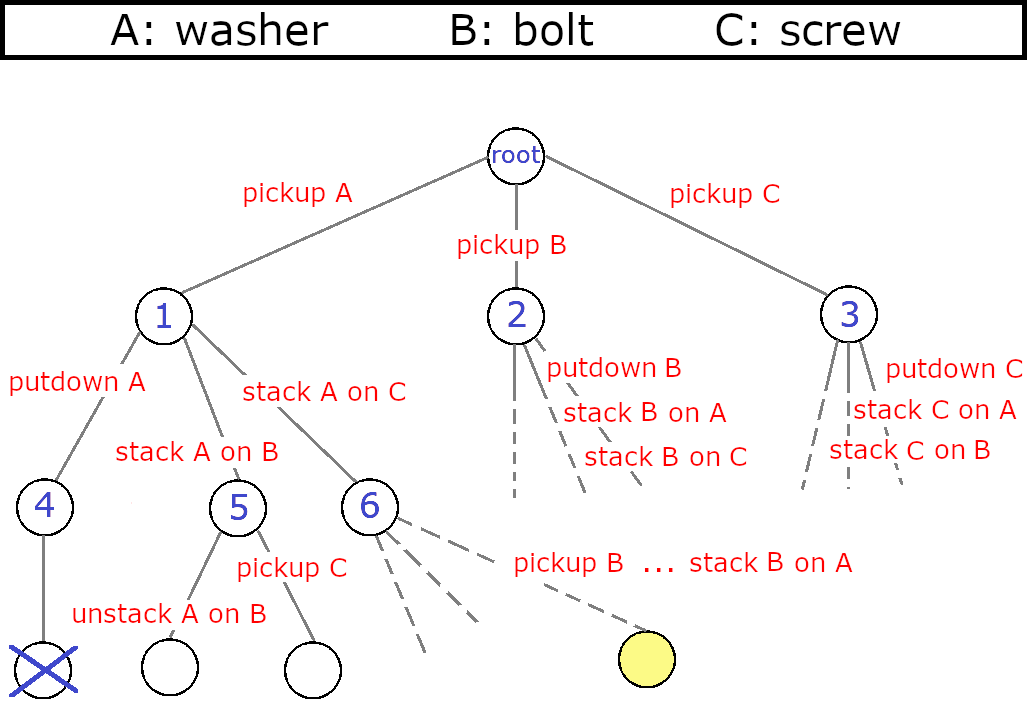
\includegraphics[width=1.0
\textwidth]{figures/Magistrale/BFS_1_blue}
\caption[BFS Example]{ TODO: descrizione
\label{fig:BFS_1}}
\end{figure} 

\section{Results Execution Phase}\label{sec:results_exec}


\begin{comment}
\begin{footnotesize}
\textbf{Code in Atomese notation:} \\
Learning phase
\end{footnotesize}

\begin{python}
	The English sentence: "The apple is in hand. The tray is on the table. The table is a fixed object."

---------------- Result:
\begin{python}
\begin{footnotesize}
\textbf{Code in Atomese notation:} \\
\textit{Pickup} action rule.
\end{footnotesize}

\begin{python}
	The English sentence: "The apple is in hand. The tray is on the table. The table is a fixed object."

---------------- Result:
\begin{python}
\end{comment}